%\addcontentsline{toc}{chapter}{Development Process}
\chapter{Software Process}

I followed an Agile approach in my project because the requirements for my project evolved as I progressed. As I researched more and learnt more about the area I had more ideas about what I wanted to include and having an Agile approach allowed me to incorporate these ideas. 

At the start of my project I drew up a rough weekly plan that would guide me through the project and allow me to see how I was progressing overall, this can be seen in figure\ref{fig:initial_weekly_plan}. This plan was useful for me to start getting an overall idea of the scope of the project and allowed me to start to split the project up into separate sections.

For the first week I followed the Kanban process and used the online tool Glo Boards\cite{glo_board}, I however quickly realised that Kanban was not the right process to use because it is generally about improving an already established process and as I was just starting I didn't have a process to improve so it didn't make a huge amount of sense to follow. 

I soon switched to using Scrum, this made a lot more sense because the project generally follows the design of a Scrum project already. I had sprints that lasted a week because each week I would have a meeting with my supervisor and I considered this meeting to be a sort of extended stand-up, I discussed and demoed what I had worked on and we discussed what I could get done by next week. The product owner was me because I was ultimately in charge of the direction of the project and what new areas it would cover, my supervisor obviously had a guiding hand in what would be developed each week and what good progress would be.

When I switched to Scrum I realised that Glo Boards weren't really working for me so I switched to using Jira\cite{jira_site}. I made heavy use of epics to group my work and epics didn't work the way I wanted them to in Glo Boards. Jira was a tool that I used during my Industrial Year and I felt that it was very useful in planning and keeping track of work. I organised my work into epics and through the use of the backlog tool and the sprint management tool it was easy to see how well I was progressing and what still needed to be done. Figure \ref{fig:jira_epics} shows how Jira lays out epics in its road map view.

\begin{figure}
    \centering
    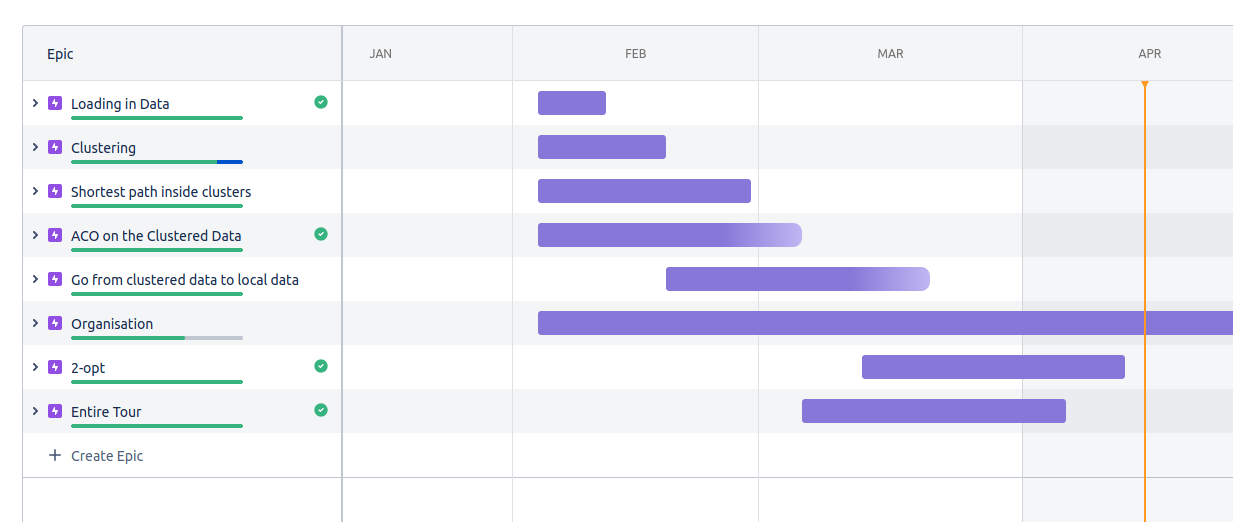
\includegraphics[width=\textwidth]{figures/jira_epics.png}
    \caption{Figure showing how the work was divided into epics in Jira, each epic had a number of tasks associated to it, when all of these tasks where completed the epic could be then be marked as done. This image was taken late into the project when most of the work had been done.}
    \label{fig:jira_epics}
\end{figure}

In Jira I assigned each task a story point estimate, this was a number between 0 and 3 that represented how much work that task would be to accomplish, 0 being very little work and 3 being a substantial amount of work normally several days. In Jira I could then generate a burndown report which could visualise how many story points I process through in a sprint and whether I was assigning myself a good amount of work each sprint. figure \ref{fig:jira_burndown} shows how this burndown chart looks in Jira.

\begin{figure}[h]
    \centering
    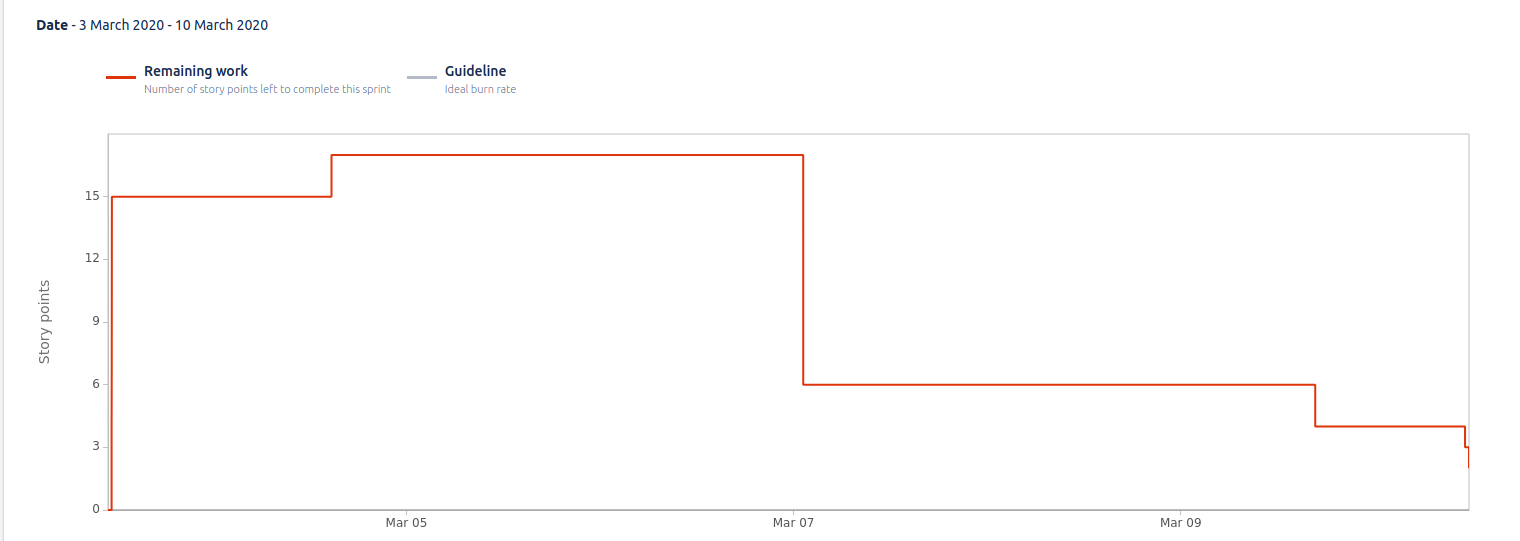
\includegraphics[width=\textwidth]{figures/jira_sprint_burndown.png}
    \caption{A Sprint burndown chart in Jira, this allows you to visualise how much work you normally accomplish on a given sprint and allow you to better plan your future sprints by allocating an appropriate amount of work. You can see in this sprint I started with 15 story points but after re-estimating a task that was raised to 17, I then managed to do most of that work and ended the sprint with 1 task left that had a story point estimate of 2.}
    \label{fig:jira_burndown}
\end{figure}

\begin{figure}[h]
    \centering
    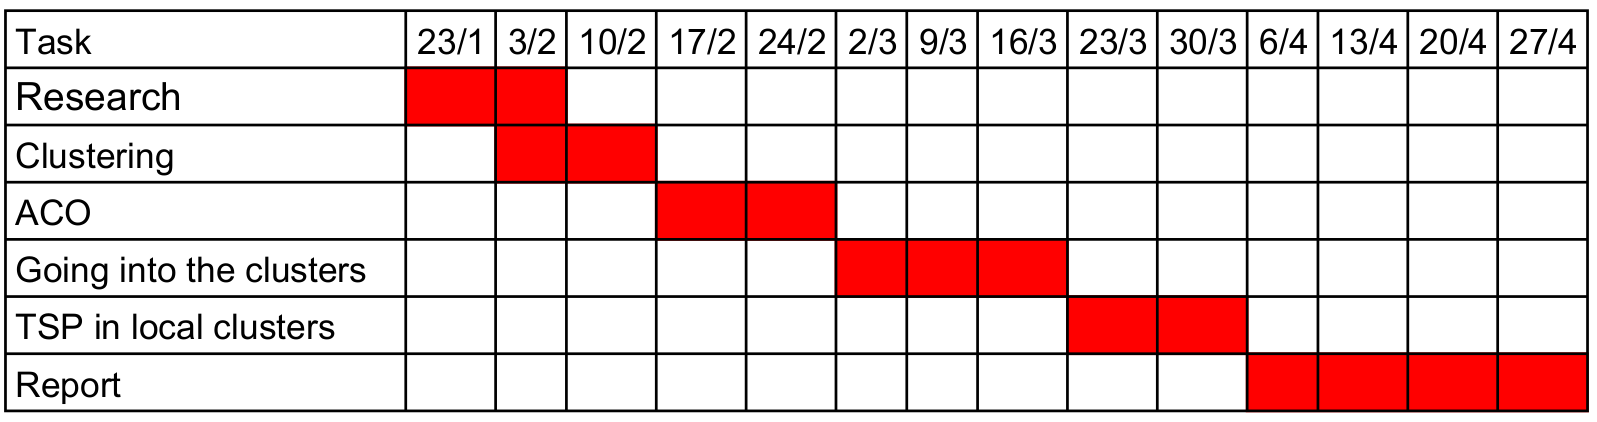
\includegraphics[width=\textwidth]{figures/initial_weekly_plan.png}
    \caption{My initial weekly plan for the project, this was just a guiding view of the project. This was meant as a way for me to monitor my progress, because I was using an Agile approach I didn't update this to include the deadline extension.}
    \label{fig:initial_weekly_plan}
\end{figure}